\section{Efficiency of the Soft Lepton tagger}

In this section we use the System8 method to measure the efficiency of a 
simple Soft Lepton Tagger (SLT) given by a cut on the \ptrel distribution of the 
muon. To ensure that the two taggers are independent and the correlation 
coefficients are close to unity, we modified the Track Counting tagger.
In the Track Counting tagger for each selected track in a jet, the impact 
parameter significance is computed. The jet is tagged by the Track Counting 
algorithm if the number of tracks with an impact parameter significance 
exceeding a given cut is greater than a discriminator value.

To create a life time tagger not involving the muon track we modified 
the jet track associator. The Jet track associator  loops over all the jets 
in an event and associates the tracks to a jet if they lie within a cone of 
0.5. We modify the Jet track associator to look for the good muons using the
criteria.
\begin{itemize} 
\item   number of Hits in the track $ \ge $ 8;
\item   $\mu $ Pt $ \ge $ 6;
\item   normalized $\chi^{2} \le 5$,
\end{itemize}   
and reject the good muon tracks from the track collection and associate rest 
of the tracks to jets. The modified jets with no muon tracks are then used 
for Track Counting method giving a modified Track counting b-tagging algorithm.

Figure~\ref{fig:Performanceplot} shows the performance plots
 comparing the modified Track Counting tagger with the Track Counting tagger
for the QCD RECO sample in the \pt range 80 to 120 GeV. Even though the 
performance of the Modified Track Counting is somewhat worse, its seperation
power is still sufficient to enrich the sample in b-jets and allow us to use 
System8 to measure the efficiency of the SLT algorithm.


\begin{figure}[htbp]
  \begin{center}
    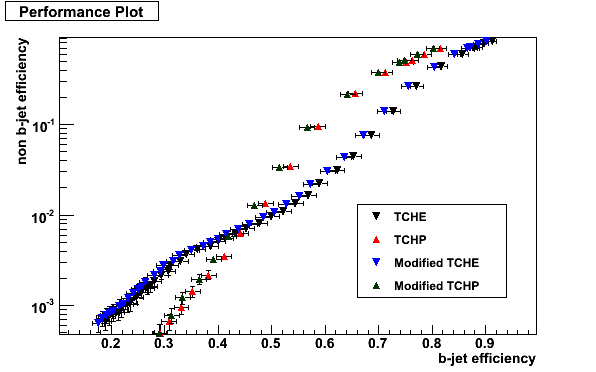
\includegraphics[width=90mm]{Figures/QCD_80_120.png}
  \end{center}
  \caption{Performance Plot comparing the performance of the default and 
modified Track Counting Algorithm for QCD 80-120 GeV sample.}
  \label{fig:Performanceplot}
\end{figure}


The Modified Track Counting tagger has been used as one of the taggers of
System8 to determine the efficiency for the Soft Lepton Tagger




